%%%%%%%% ICML 2026 EXAMPLE LATEX SUBMISSION FILE %%%%%%%%%%%%%%%%%

\documentclass{article}

\usepackage{microtype}
\usepackage{graphicx}
\usepackage{subcaption}
\usepackage{booktabs}
\usepackage{hyperref}
\usepackage{amsmath}
\usepackage{amssymb}
\usepackage{mathtools}
\usepackage{amsthm}
\usepackage[capitalize,noabbrev]{cleveref}

\newcommand{\theHalgorithm}{\arabic{algorithm}}

\usepackage{icml2026}

\icmltitlerunning{m2sv: Map-to-Street-View Spatial Reasoning Benchmark}

\begin{document}

\twocolumn[
\icmltitle{m2sv: A Scalable Benchmark for Map-to-Street-View Spatial Reasoning}

\icmlsetsymbol{equal}{*}

\begin{icmlauthorlist}
  \icmlauthor{Firstname1 Lastname1}{equal,yyy}
  \icmlauthor{Firstname2 Lastname2}{equal,yyy,comp}
\end{icmlauthorlist}

\icmlaffiliation{yyy}{Department of XXX, University of YYY, Location, Country}
\icmlaffiliation{comp}{Company Name, Location, Country}

\icmlcorrespondingauthor{Firstname1 Lastname1}{first1.last1@xxx.edu}

\icmlkeywords{vision-language models, spatial reasoning, geospatial understanding}

\vskip 0.3in
]

\printAffiliationsAndNotice{}

% ===============================================================
\begin{abstract}
Vision--language models (VLMs) have achieved strong performance on many multimodal
benchmarks but remain brittle on spatial reasoning tasks that require aligning
abstract overhead representations with egocentric views. We introduce
\textbf{m2sv}, a scalable benchmark for map-to-street-view spatial reasoning that
asks models to infer camera viewing direction by aligning a north-up overhead map
with a Street View image captured at the same physical location. The released
\textbf{m2sv-20k} benchmark contains 20,000 intersection-based examples with
controlled ambiguity and geographic diversity, and we additionally provide
\textbf{m2sv-sft-11k}, a curated set of structured reasoning traces for supervised
fine-tuning. Despite strong performance on many multimodal benchmarks, the best
evaluated VLM reaches only 57.2\% accuracy on m2sv, far below the human baseline
of 88\%. While supervised fine-tuning and reinforcement learning improve
performance, cross-benchmark experiments reveal limited transfer. These results
highlight persistent gaps in geometric alignment and motivate further research
on grounded spatial reasoning.
\end{abstract}

% ===============================================================
\section{Introduction}

Vision--language models have demonstrated impressive capabilities in object
recognition, diagram understanding, and text-heavy multimodal reasoning.
However, they continue to struggle with tasks that require consistent spatial
grounding across viewpoints. In particular, aligning abstract overhead
representations such as maps with egocentric, ground-level imagery remains a
fundamental challenge. This capability underlies applications in navigation,
robotics, and embodied assistants, yet is weakly represented in existing
benchmarks.

Most multimodal reasoning benchmarks emphasize synthetic diagrams, charts, or
curated visual puzzles where geometry is simplified or explicitly annotated.
Real-world spatial reasoning introduces additional complexity: viewpoint changes,
partial observability, temporal mismatch between data sources, and ambiguous or
transient visual cues. As a result, current benchmarks may overestimate spatial
competence by avoiding alignment between disparate viewpoints.

We introduce \textbf{m2sv} (map-to-street-view), a benchmark designed to isolate a
core spatial reasoning primitive: inferring camera viewing direction by aligning
a north-up overhead map with a Street View image captured at a real-world
intersection. Each example requires reasoning about road topology, intersection
geometry, and stable landmarks, while ignoring transient elements such as
vehicles or pedestrians.

Our contributions are:
\begin{itemize}
  \item A fully automated pipeline for constructing large-scale map-to-street-view
  spatial reasoning benchmarks.
  \item \textbf{m2sv-20k}, a geographically diverse benchmark with controlled
  ambiguity and statistically reliable evaluation.
  \item \textbf{m2sv-sft-11k}, a curated set of structured reasoning traces for
  supervised fine-tuning.
  \item An extensive evaluation revealing large gaps between VLMs and human
  performance, modest gains from adaptation, and limited cross-benchmark transfer.
\end{itemize}

% ===============================================================
\section{Benchmark Design}

Each m2sv example consists of two images: (1) a north-up overhead map centered at
a real-world intersection, annotated with labeled directional rays, and (2) a
Street View image captured near the same intersection and oriented along one of
those rays. The task is to identify which labeled direction corresponds to the
Street View camera orientation.

The number of candidate directions per example ranges from 2 to 7, with a median
of 3 (mean: 3.24). Accordingly, the random-guess baseline is approximately
31.7\%. Accuracy is measured over multiple-choice labels.

\begin{figure*}[t]
  \centering
  \begin{subfigure}[t]{0.48\linewidth}
    \centering
    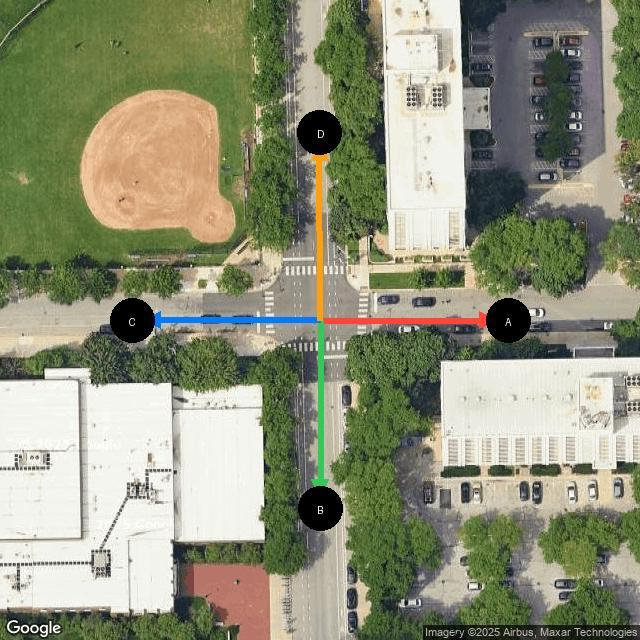
\includegraphics[width=\linewidth]{figures/sample-question-1-map.jpg}
    \caption{North-up overhead map with labeled candidate directions.}
    \label{fig:m2sv-example-map}
  \end{subfigure}\hfill
  \begin{subfigure}[t]{0.48\linewidth}
    \centering
    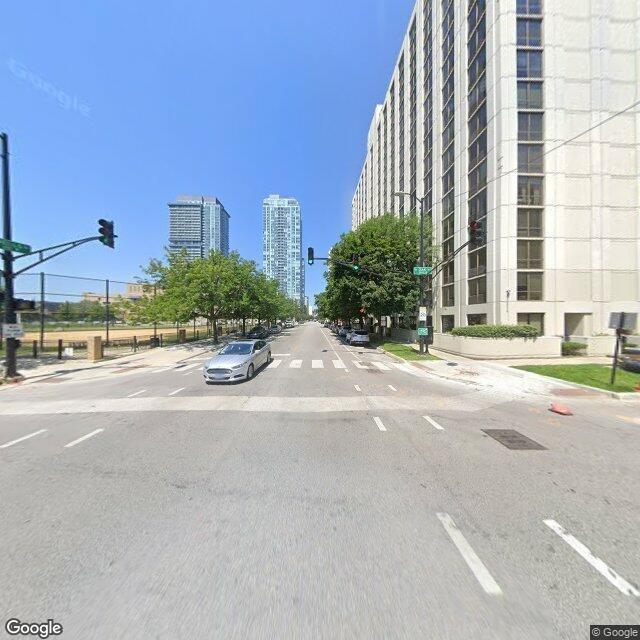
\includegraphics[width=\linewidth]{figures/sample-question-1-sv.jpg}
    \caption{Street View image captured at the same intersection.}
    \label{fig:m2sv-example-sv}
  \end{subfigure}

  \vspace{0.75em}
  \begin{minipage}{0.98\linewidth}
    \footnotesize
    \begin{tabular}{p{0.96\linewidth}}
      \toprule
      \textbf{Question} \\
      Which labeled direction on the map corresponds to the direction in which the street view photo was taken? Options: A, B, C, D. \\
      \midrule
      \textbf{Generated trace (Gemini-2.5-Pro)} \\
      \textbf{Step 1: Analyze the street-view photo.} The photo is taken from the center of an intersection, looking straight ahead. On the immediate right is a very tall, light-colored (white or beige) apartment or office building. It runs along the street from the corner onwards. On the immediate left is a fenced-off open area, which looks like a park or a sports field. There are trees lining the sidewalk. In the distance, further down the road, at least two prominent skyscrapers are visible. The road itself is a multi-lane street. \\
      \textbf{Step 2: Analyze the overhead map and evaluate each option.} The camera is at the central intersection. Option A (looking East): To the right (south) is a large white building. To the left (north) is another large white building. This does not match the photo, which has a park/field on the left. Option B (looking South): To the right (west) is a large white building. To the left (east) is another large white building. This does not match the photo. Option C (looking West): To the right (north) is a large green area with a baseball field. To the left (south) is a large white building. This is the opposite of the street view (building on the right, park on the left). Option D (looking North): To the right (east) is a long, rectangular, light-colored building located right at the corner. To the left (west) is a large green area containing a baseball field. This arrangement perfectly matches the street-view photo. \\
      \textbf{Step 3: Conclude the comparison.} Direction D is the only view from the intersection that has a large park/baseball field on the left and a tall, long building on the right. Final answer: \textbackslash boxed\{D\}. \\
      \midrule
      \textbf{Ground truth} \\
      D \\
      \bottomrule
    \end{tabular}
  \end{minipage}

  \caption{Illustrative m2sv example with paired images and a model-generated
  reasoning trace. The model correctly infers the viewing direction by aligning
  stable map geometry with the Street View image.}
  \label{fig:m2sv-example}
\end{figure*}

% ===============================================================
\section{Dataset and Blueprint Pipeline}

\subsection{Blueprint specification}

We decouple dataset specification from image rendering by releasing blueprint
metadata that records intersection coordinates, candidate azimuths, correct
labels, and Street View panorama identifiers. Images are rendered on demand using
a standardized pipeline, enabling deterministic reconstruction of the dataset.

\subsection{Sampling and filtering}

Intersections are sampled from a seed list of major metropolitan areas worldwide
to encourage broad geographic coverage. The sampling pipeline itself is
city-agnostic and can be readily extended to additional regions by modifying the
city list.

To control ambiguity and ensure fair evaluation, we apply several filtering
criteria. Street View panoramas are restricted to within 5 m of the intersection
center, resulting in a tightly controlled offset distribution (median: 2.05 m;
95th percentile: 4.51 m). We further enforce a minimum angular separation of 15°
between candidate azimuths to exclude near-collinear road configurations that are
difficult even for humans to disambiguate.

\subsection{Dataset statistics}

m2sv-20k contains 20,000 examples spanning 32 cities across multiple continents.
Per-city caps prevent over-representation of dense urban areas. The number of
candidate directions per example ranges from 2 to 7 (min: 2, max: 7, mean: 3.24,
median: 3).

\begin{table}[t]
  \centering
  \caption{Summary statistics of the m2sv-20k dataset.}
  \label{tab:dataset-stats}
  \begin{tabular}{l r}
    \toprule
    Statistic & Value \\
    \midrule
    Number of examples & 20,000 \\
    Number of cities & 32 \\
    Candidate directions (median) & 3 \\
    Street View distance (median) & 2.05 m \\
    Street View distance (95\%) & 4.51 m \\
    \bottomrule
  \end{tabular}
\end{table}

\subsection{Reasoning traces}

We curate \textbf{m2sv-sft-11k}, a subset of 11,000 examples annotated with
structured reasoning traces generated by a strong proprietary model. Traces
explicitly compare map geometry and Street View imagery and terminate in a boxed
final answer. These traces are used exclusively for supervised fine-tuning
experiments.

% ===============================================================
\section{Experimental Setup}

We evaluate a range of proprietary and open-source VLMs using a standardized
prompt that describes the task and instructs models to ignore transient visual
elements. Accuracy and 95\% confidence intervals are reported.

Supervised fine-tuning uses m2sv-sft-11k. Reinforcement learning experiments build
on SFT models using HF GRPOTrainer with default DAPO settings.

% TODO: Move prompt template and full hyperparameters to appendix.

% ===============================================================
\section{Results}

\subsection{Zero-shot baselines and human gap}

\begin{table}[t]
  \centering
  \caption{Zero-shot baseline performance on m2sv with 95\% confidence intervals.}
  \label{tab:m2sv-baselines}
  \begin{tabular}{l r r}
    \toprule
    Model & N & Accuracy (\%) \\
    \midrule
    GPT-5 & 1k & 57.2 $\pm$ 3.1 \\
    Gemini-2.5-Pro & 1k & 47.2 $\pm$ 3.1 \\
    \midrule
    Qwen3-VL-8B-Instruct & 1k & 35.5 $\pm$ 3.0 \\
    Qwen3-VL-32B-Thinking & 1k & 40.7 $\pm$ 3.1 \\
    \midrule
    Random baseline & 10k & 31.7 $\pm$ 0.9 \\
    Human baseline & 100 & 88.0 $\pm$ 6.4 \\
    \bottomrule
  \end{tabular}
\end{table}

Even the strongest evaluated model performs far below humans, while most open
models operate near the random baseline.

\subsection{Adaptation baselines}

\begin{table}[t]
  \centering
  \caption{Adaptation results on m2sv-20k (10k validation).}
  \label{tab:m2sv-main-results}
  \begin{tabular}{l l r}
    \toprule
    Model & Training & Accuracy (\%) \\
    \midrule
    Qwen3-VL-8B & Base & 34.3 $\pm$ 0.9 \\
    Qwen3-VL-8B & SFT & 39.8 $\pm$ 1.0 \\
    Qwen3-VL-8B & SFT+RL & 43.9 $\pm$ 1.0 \\
    \bottomrule
  \end{tabular}
\end{table}

Supervised fine-tuning and reinforcement learning yield consistent gains, but a
substantial gap to human performance remains.

\subsection{Cross-benchmark transfer}

\begin{table*}[t]
  \centering
  \caption{Cross-benchmark evaluation for Qwen3-VL-8B variants.}
  \label{tab:transfer}
  \begin{tabular}{l c c c c c}
    \toprule
    Model & MMMU & MME-Cog & MME-Per & MMStar & Omni3D \\
    \midrule
    Base & 0.556 & 643 & 1721 & 0.604 & 0.388 \\
    SFT & 0.574 & 501 & 1525 & 0.574 & 0.372 \\
    SFT+RL & 0.563 & 550 & 1670 & 0.644 & -- \\
    \bottomrule
  \end{tabular}
\end{table*}

Transfer across benchmarks is mixed and sensitive to prompting format, suggesting
limited generalization of spatial representations.

% ===============================================================
\section{Analysis}

\paragraph{Failure analysis.}
% TODO: Add error taxonomy table and qualitative examples.

\paragraph{Difficulty slicing.}
% TODO: Slice accuracy by number of options, Street View distance, and
% intersection degree.

\paragraph{Human vs model errors.}
% TODO: Compare representative human and model failure cases.

% ===============================================================
\section{Limitations and Societal Impact}

m2sv relies on the availability and coverage of commercial mapping services and
reflects biases in their data collection. The benchmark focuses exclusively on
public road intersections and does not include private or sensitive locations.

% ===============================================================
\section{Conclusion}

m2sv provides a scalable benchmark for evaluating map-to-street-view spatial
reasoning under real-world conditions. Despite advances in multimodal modeling,
substantial gaps remain between VLMs and human performance. By isolating a core
geometric alignment task and enabling large-scale evaluation, m2sv offers a
useful diagnostic tool for future research on grounded spatial reasoning.

\bibliographystyle{icml2026}

\end{document}